%22/10 - Paco Jurado
\chapter{Procesamiento de lenguaje natural}
\section{Procesado de lenguaje natural}
\subsection{Definición de PLN}
El procesamiento del lenguaje natural (NLP por sus siglas en inglés) son un conjunto de métodos para hacer el lenguaje humano accesible a los ordenadores. Así, permite una comunicación "natural" entre humanos y máquinas y mejora la comunicación entre humanos (por ejemplo por traducción).

La ciencia ficción ya mostraba desde finales de los 70 máquinas que podían hablar. 

\subsection{Desafíos del NLP}
El test de Turing lo desarrolló Alan Turing en 1950 para comprobar la capacidad de una máquina a mantener una conversación como si fuera un humano. El test se basa en un humano que "chattea" y debe distinguir si está hablando con otro humano o con una máquina. Si no lo puede distinguir, se considera que la máquina ha pasado el test de Turing. 

NLP es difícil porque los lenguajes humanos son ambiguos, ilimitados, diversos, difusos, más y menos articulados. Hay palabras polisémicas, el orden de las palabras afecta a su significado, expresiones hechas ("dame tu teléfono" no se refiere al dispositivo, si no al número). La ambigüedad sintáctica se puede dar por la sintaxis, referencias a pronombres, y aunque para los humanos sea fácil de detectar y forme la base de muchos chistes, a la hora de pasarlo a la máquina se convierte en un problema. 

A la hora de hacer las traducciones, depende la composición de palabras. Dos palabras que por separado tienen un significado, cuando están juntas pueden tener otro. 

\subsection{Interdisciplinariedad del NLP}
El NLP se basa en muchas disciplinas muy diversas. Están los \textbf{lingüistas}, que buscan analizar cómo funciona el lenguaje, los ingenieros en \textbf{machine learning} e \textbf{inteligencia artificial} para poder automatizar las tareas y crear programas complejos. En general, toda la \textbf{informática} presenta la base de los algoritmos utilizados en NLP.

Estas áreas son las que diseñan los primeros algoritmos, pero con el tiempo salen cuestiones \textbf{sociales y éticas} por sesgos sociales, como pueden ser los géneros al traducir del inglés al español (nurse se traducía sólo como enfermera, no salía la alternativa de enfermero).

\section{Aplicaciones prácticas}
Entre las aplicaciones del NLP se encuentran:
\begin{itemize}
\item Traducción automática: traducción de un texto de un idioma a otro en su significado (no palabra por palabra).
\item Obtención de información: dada una consulta en nuestro idioma, identifica los documentos y páginas relevantes para esa búsqueda. 
\item Extracción de información: se tienen documentos de texto que no están estructurados (en cuanto a información, no del texto) de los cuales se intenta extraer la información estructurada para una base de datos.
\item Respuesta a preguntas: responder automáticamente preguntas propuestas por humanos en base a la información ya almacenada.
\item Clasificación de texto: asigna categorías o tags a textos en base a su contenido.
\item Minería de opiniones y análisis de sentimientos: identificar, extraer, cuantificar y estudiar de forma sistemática los estados afectivos y la información subjetiva (a partir del contenido textual generado por los usuarios).
\item Sistema de diálogo: Un agente conversacional o chatbot es un sistema informático diseñado para conversar con un ser humano (a través de un canal de texto). Los asistentes virtuales/personales inteligentes pueden realizar tareas o prestar servicios a una persona basándose en órdenes o preguntas. Así se crearon los agentes de generación de lenguaje conversacionales como ChatGPT o Gemini. Estos algoritmos generan texto como lo haría un humano (o como se ha hecho previamente), y estos sí pasan el test de Turing.
\end{itemize}

\section{Niveles del análisis lingüístico y tareas NLP}
\subsection{El pipeline de NLP}
Para conocer un idioma, hay que manejar muchos niveles de análisis lingüístico: habla, fonética, ortografía, morfología, lexemas, sintaxis, semántica, pragmática, etc. 

\begin{figure}[h]
\centering
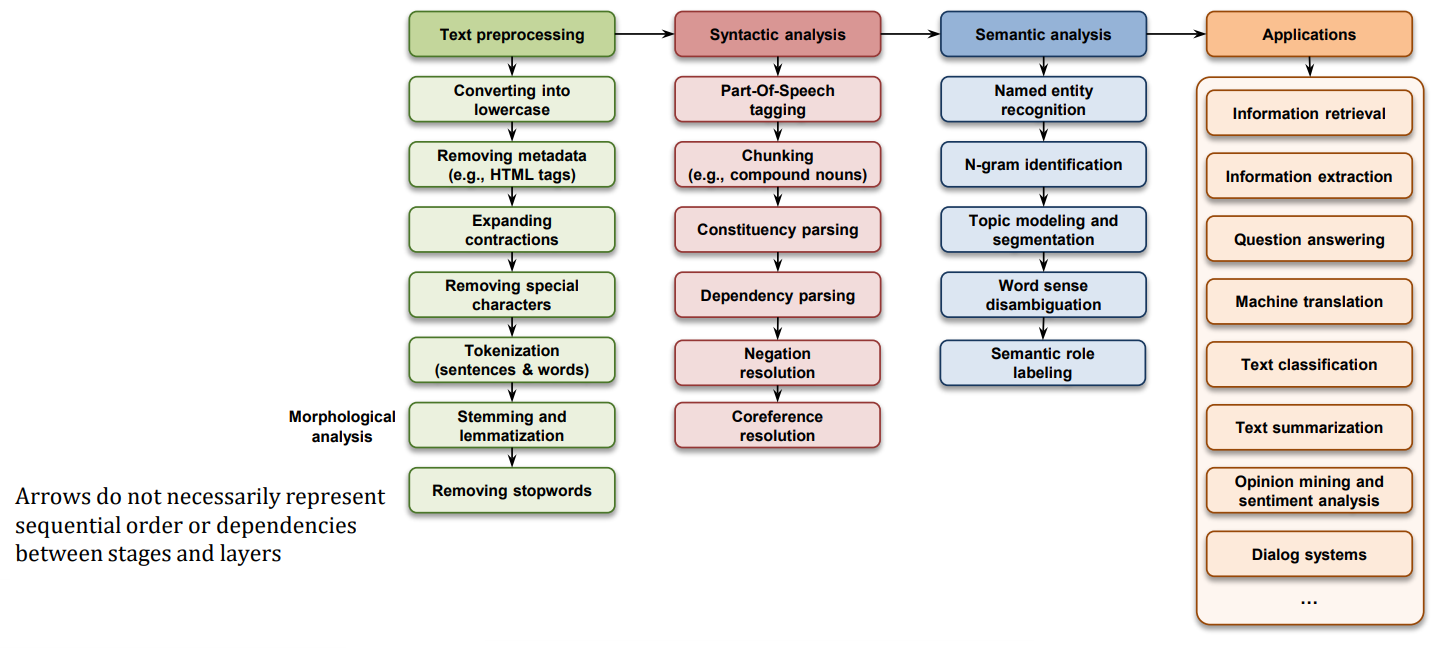
\includegraphics[width = \textwidth]{figs/nlp-pipeline.png}
\end{figure}

El primer paso es el \textbf{preprocesamiento} para normalizar todo (pasar a minúscula), quitar la metadata (tags, html), expandir las contracciones o los acrónimos, eliminar caracteres especiales, etc. También se eliminan las stopwords, que son palabras que no aportan nada de información, como los artículos o los verbos auxiliares. A continuación se stemiza y lematiza, es decir, se quitan las conjugaciones para obtener la raíz y obtener el lema (la palabra normalizada).

El siguiente paso es el \textbf{análisis sintáctico} donde se identifican las partes de la oración, se hace una composición de los grupos (nominales, preposicionales, etc) donde entra el análisis de constituyentes, resolución de dependencias y negaciones y se entra al \textbf{análisis semántico}. Con todo el procesamiento se pasan a las \textbf{aplicaciones}.

\subsection{Análisis sintáctico}
\paragraph{Part-Of-Speech (POS) tagging}
El POS tagging identifica para cada palabra o token si se trata de un nombre propio, verbo, determinante, etc. 

\paragraph{Parseo de constituyentes}
Las palabras tienen su POS tag y se van agrupando las estructuras sintácticas.

\paragraph{Parseo de dependencias}
Se extrae la estructura gramática de una oración, buscando la relación entre los constituyentes definidos previamente. 

\subsection{Análisis semántico}
\paragraph{Named Entity Recognition (NER)}
El reconocimiento de entidades se utiliza mucho en distintos contextos. Busca reconocer localizaciones, personas, lugares geopolíticos, números de teléfono, fechas, etc. Esto se puede utilizar posteriormente para la extracción de información. 

\paragraph{Resolución de co-referencias}
Se busca qué hace referencia a la misma entidad en un texto para reemplazarlo y que el procesamiento del texto sea igual. En ocasiones, es necesario completar la información (por ejemplo, una noticia de "el presidente ha dicho ...", si a la semana hay un cambio de gobierno).

\paragraph{Word Sense Disambiguation (WSD)}
En ocasiones, las palabras pueden hacer referencia a más de una cosa por ser polisémicas o tener otras ambigüedades, por lo que se deben desambigüar. Para ello se debe ver el contexto de la oración. Generalmente, se coge la palabra de la frase con menos alternativas de ambigüedades y a partir de ella se escogen las otras acepciones.

\paragraph{Etiquetado semántico}
Al hacer el etiquetado semántico, se le está poniendo cierta taxonomía para indicar las estructuras predicado-argumento como agente, predicado, tema y localización. Son representaciones abstractas de las funciones.

\section{Breve historia del NLP}
\subsection{NLP antes de la era Deep Learning}
Los inicios se deben a lingüistas y matemáticos. En los 1960s, se formalizan las teorías gramáticas. En los 90 se generan modelos estadísticos que permitieron identificar los stopwords en base a la frecuencia. Los modelos bayesianos funcionaban muy bien.

\subsection{NLP durante la era Deep Learning}
Los primeros modelos neuronales aplicados al lenguaje entraron en el 2003 y requerían una computación enorme. En los 2010 se crearon las GPU, por lo que el tratamiento matricial mejoró con creces. También entraron los word embedding, donde se obtenían representaciones vectoriales de los conceptos vinculados a las palabras con redes neuronales. Esto marcó un antes y un después. Se crearon distintas arquitecturas con los mecanismos de atención y transformer, y en 2020 los modelos grandes de lenguaje.

Muchos de los modelos creados antes de la era Deep Learning se siguen utilizando hoy día. Si por la tarea no se requiere una arquitectura deep, se pueden utilizar los modelos "clásicos". 